\documentclass[final,3p,times]{elsarticle}

%% Use the option review to obtain double line spacing
%% \documentclass[authoryear,preprint,review,12pt]{elsarticle}

%% Use the options 1p,twocolumn; 3p; 3p,twocolumn; 5p; or 5p,twocolumn
%% for a journal layout:
%% \documentclass[final,1p,times]{elsarticle}
%% \documentclass[final,1p,times,twocolumn]{elsarticle}
%% \documentclass[final,3p,times]{elsarticle}
%% \documentclass[final,3p,times,twocolumn]{elsarticle}
%% \documentclass[final,5p,times]{elsarticle}
%% \documentclass[final,5p,times,twocolumn]{elsarticle}

%% For including figures, graphicx.sty has been loaded in
%% elsarticle.cls. If you prefer to use the old commands
%% please give \usepackage{epsfig}

%% The amssymb package provides various useful mathematical symbols
\usepackage{amssymb}
%% The amsmath package provides various useful equation environments.
\usepackage{amsmath}
\usepackage{hyperref}
%% The amsthm package provides extended theorem environments
%% \usepackage{amsthm}

%% The lineno packages adds line numbers. Start line numbering with
%% \begin{linenumbers}, end it with \end{linenumbers}. Or switch it on
%% for the whole article with \linenumbers.
%% \usepackage{lineno}

\usepackage{array}
\usepackage{booktabs}
\usepackage{multirow}
\usepackage{microtype}
\usepackage{siunitx}
\usepackage{url}

\journal{Computers and Electronics in Agriculture}
\graphicspath{{figures/final/}}

\renewcommand\floatpagefraction{.9}
\renewcommand\topfraction{.9}
\renewcommand\bottomfraction{.9}
\renewcommand\textfraction{.1}
\setcounter{totalnumber}{50}
\setcounter{topnumber}{50}
\setcounter{bottomnumber}{50}

\begin{document}

\begin{frontmatter}

\title{AFMS: a minimal-protocol-driven framework for multi-species aquaculture animal phenotyping}

\author[label1,label2]{Cheng-long Zhang\corref{+}}
\author[label1,label2]{Jihu Zhang\corref{+}}
\author[label1,label2]{Yongzheng Wang}
\author[label1,label2]{Yu Cheng}
\author[label1,label2]{Haochen Jiang}
\author[label1,label2]{Ziyan Jin}
\author[label1,label2]{Kairu Zhang}
\author[label1,label2]{Xiang Shan Ji\corref{*}}
\author[label1,label2]{Yan Zhao\corref{*}}

\ead{xsji@sdau.edu.cn, yzhao@sdau.edu.cn}

\cortext[+]{These authors contributed equally to this work.}
\cortext[*]{Corresponding author(s)}

\affiliation[label1]{
  organization={Key Laboratory of Efficient Utilization of Non-grain Feed Resources (Co-construction by Ministry and Province) of Ministry of Agriculture and Rural Affairs, Shandong Agricultural University},
  city={Taian},
  state={Shandong},
  country={China}
}

\affiliation[label2]{
  organization={Shandong Provincial Key Laboratory for Livestock Germplasm Innovation \& Utilization, Shandong Agricultural University},
  city={Taian},
  state={Shandong},
  country={China}
}

\begin{abstract}
Aquaculture breeding programs require large-scale phenotyping of body morphology, appendage traits, and growth indicators across diverse species. However, different species require different anatomical landmarks, measurement traits, and quality-control rules, and existing computer-vision phenotyping tools are typically built for a single species, making adaptation to new species dependent on software redevelopment. We developed AFMS, a phenotyping framework in which species-specific measurement knowledge is externalized into a compact protocol file. Species-specific measurement definitions are encoded in approximately 20 lines of configuration, after which the framework handles detection, measurement, quality control, and data export. The same system supports five aquaculture taxa spanning three taxonomic orders without core runtime code modification, and accommodates pixel-space, physical-tag-calibrated, and structured-light 3D measurement modes. Detection mAP@0.5 ranged from 0.955 to 1.000, and four of five species achieved keypoint PCK above 0.927. An operational batch-processing test conducted by breeding practitioners on 1591 samples over 118 minutes achieved a 98.8\% success rate. These results suggest that AFMS can reduce species adaptation from software redevelopment toward protocol-level definition, providing a protocol-based route for adapting phenotyping workflows across aquaculture species without modifying the core software.
\end{abstract}

\begin{keyword}
aquaculture phenotyping \sep multi-species adaptation \sep protocol-driven phenotyping \sep keypoint detection \sep depth-aware measurement \sep batch phenotyping \sep breeding infrastructure
\end{keyword}

\end{frontmatter}

\section{Introduction}

High-throughput phenotyping has become a central requirement for linking genotype, environment, and production traits in modern biological systems \citep{houle2010phenomics}. In aquaculture breeding, phenotyping and phenomics are increasingly used to record growth, body morphology, body condition, appendage traits, and weight-linked indicators across populations and production stages \citep{fu2022phenotyping,zhao2024biotech}. These traits are repeatedly collected during selective breeding, growth monitoring, grading, and population management. As aquaculture datasets become larger and more longitudinal, phenotyping systems must support scalable acquisition, standardized records, and structured outputs that can be reused by breeding and management databases \citep{tuckey2022automated}.

Computer vision and deep learning have substantially improved the automation potential of aquaculture phenotyping. Image-based methods can extract body length from photographs \citep{strachan1993length,monkman2019machine,marrable2023generalised}, measure morphometric traits \citep{zion2012computer,navarro2016imafish,yu2023keypoint,he2024measurement}, and estimate biomass indicators \citep{saberioon2017machine,fernandes2020segmentation,liu2023objectdetection,li2020nonintrusive,zhang2024biomass}. Depth-aware systems can convert image measurements into real-space coordinates \citep{zhao2025stereo,zhou2023inwater,tonachella2022fishial}. However, these tools are typically built for a single species, a single measurement target, or a specific research workflow. In practice, different species require different anatomical landmarks: a carp needs body-axis landmarks and length-height ratios, a crab requires carapace and appendage measurements, and a crayfish may need only three landmarks on a segmented body. Existing tools cannot accommodate this diversity without per-species software redevelopment \citep{liu2024fishphenokey,he2024measurement}.

The result is a persistent gap between published methods and deployed systems \citep{liu2024fishphenokey}. When a new species needs to be measured, the required changes span annotation definitions, model configurations, inference scripts, measurement functions, quality-control logic, and export formats, all embedded in application code \citep{navarro2016imafish,fernandes2020segmentation}. Even multi-species systems such as IMAFISH\_ML still require software-level adaptation for each new species \citep{navarro2016imafish}. Per-species redevelopment remains the norm for landmark-based measurement \citep{yu2023keypoint} and depth-aware phenotyping \citep{zhao2025stereo,zhou2023inwater}. This coupling makes species adaptation dependent on software-level modification, even when the desired measurement traits are biologically simple \citep{abinaya2022segmental}.

The root cause is not insufficient model accuracy but excessive software coupling: species-specific anatomical definitions, measurement rules, quality thresholds, and output schemas are embedded in code rather than declared in a species-agnostic interface \citep{gonzalez2023phytooracle}. When the species changes, the code changes. Decoupling measurement definitions from implementation would allow a single runtime to serve multiple species.

Here we present AFMS, a phenotyping framework designed to bridge this gap. AFMS externalizes species-specific measurement knowledge into a compact protocol file. The protocol specifies what to measure (landmarks, trait connections, measurement rules, scoring weights), and the framework handles how to detect, calculate, and export. AFMS is not a new detection model or pose-estimation method; it uses established perception components \citep{lyu2022rtmdet,jiang2023rtmpose,chen2019mmdetection,mmpose,lin2014coco} as interchangeable modules. The contributions of this work are:

\begin{itemize}
  \item We propose a minimal species protocol that encodes species-specific measurement rules, including landmarks, traits, scoring, and quality-control rules, in a compact declarative file, reducing the need for species-specific core runtime code modification.
  \item We develop a shared phenotyping system in which the same software supports all species through protocol-driven configuration. Five taxa spanning three taxonomic orders use the same system without core runtime code modification.
  \item We integrate multi-modal measurement (pixel-space, physical-tag-calibrated, and structured-light 3D) within the same framework, allowing the appropriate measurement mode to be selected based on available sensor hardware.
  \item We validate AFMS across morphologically diverse aquaculture taxa and an operational batch-processing scenario involving breeding practitioners.
\end{itemize}

\section{Materials and methods}

\subsection{System overview}

AFMS is designed as an application-oriented phenotyping framework rather than as a single-species measurement script or a model benchmark (Fig.~\ref{fig:system_architecture}). The system is organized into three layers: an acquisition layer for image and depth capture, a software layer for inference, measurement, quality control, and data export, and a model layer for training and deploying perception models. A species protocol sits at the center, connecting all layers by providing species-specific measurement definitions to every module. This modular separation of concerns follows principles established in other phenotyping frameworks \citep{gonzalez2023phytooracle}.

\begin{figure}[htbp]
  \centering
  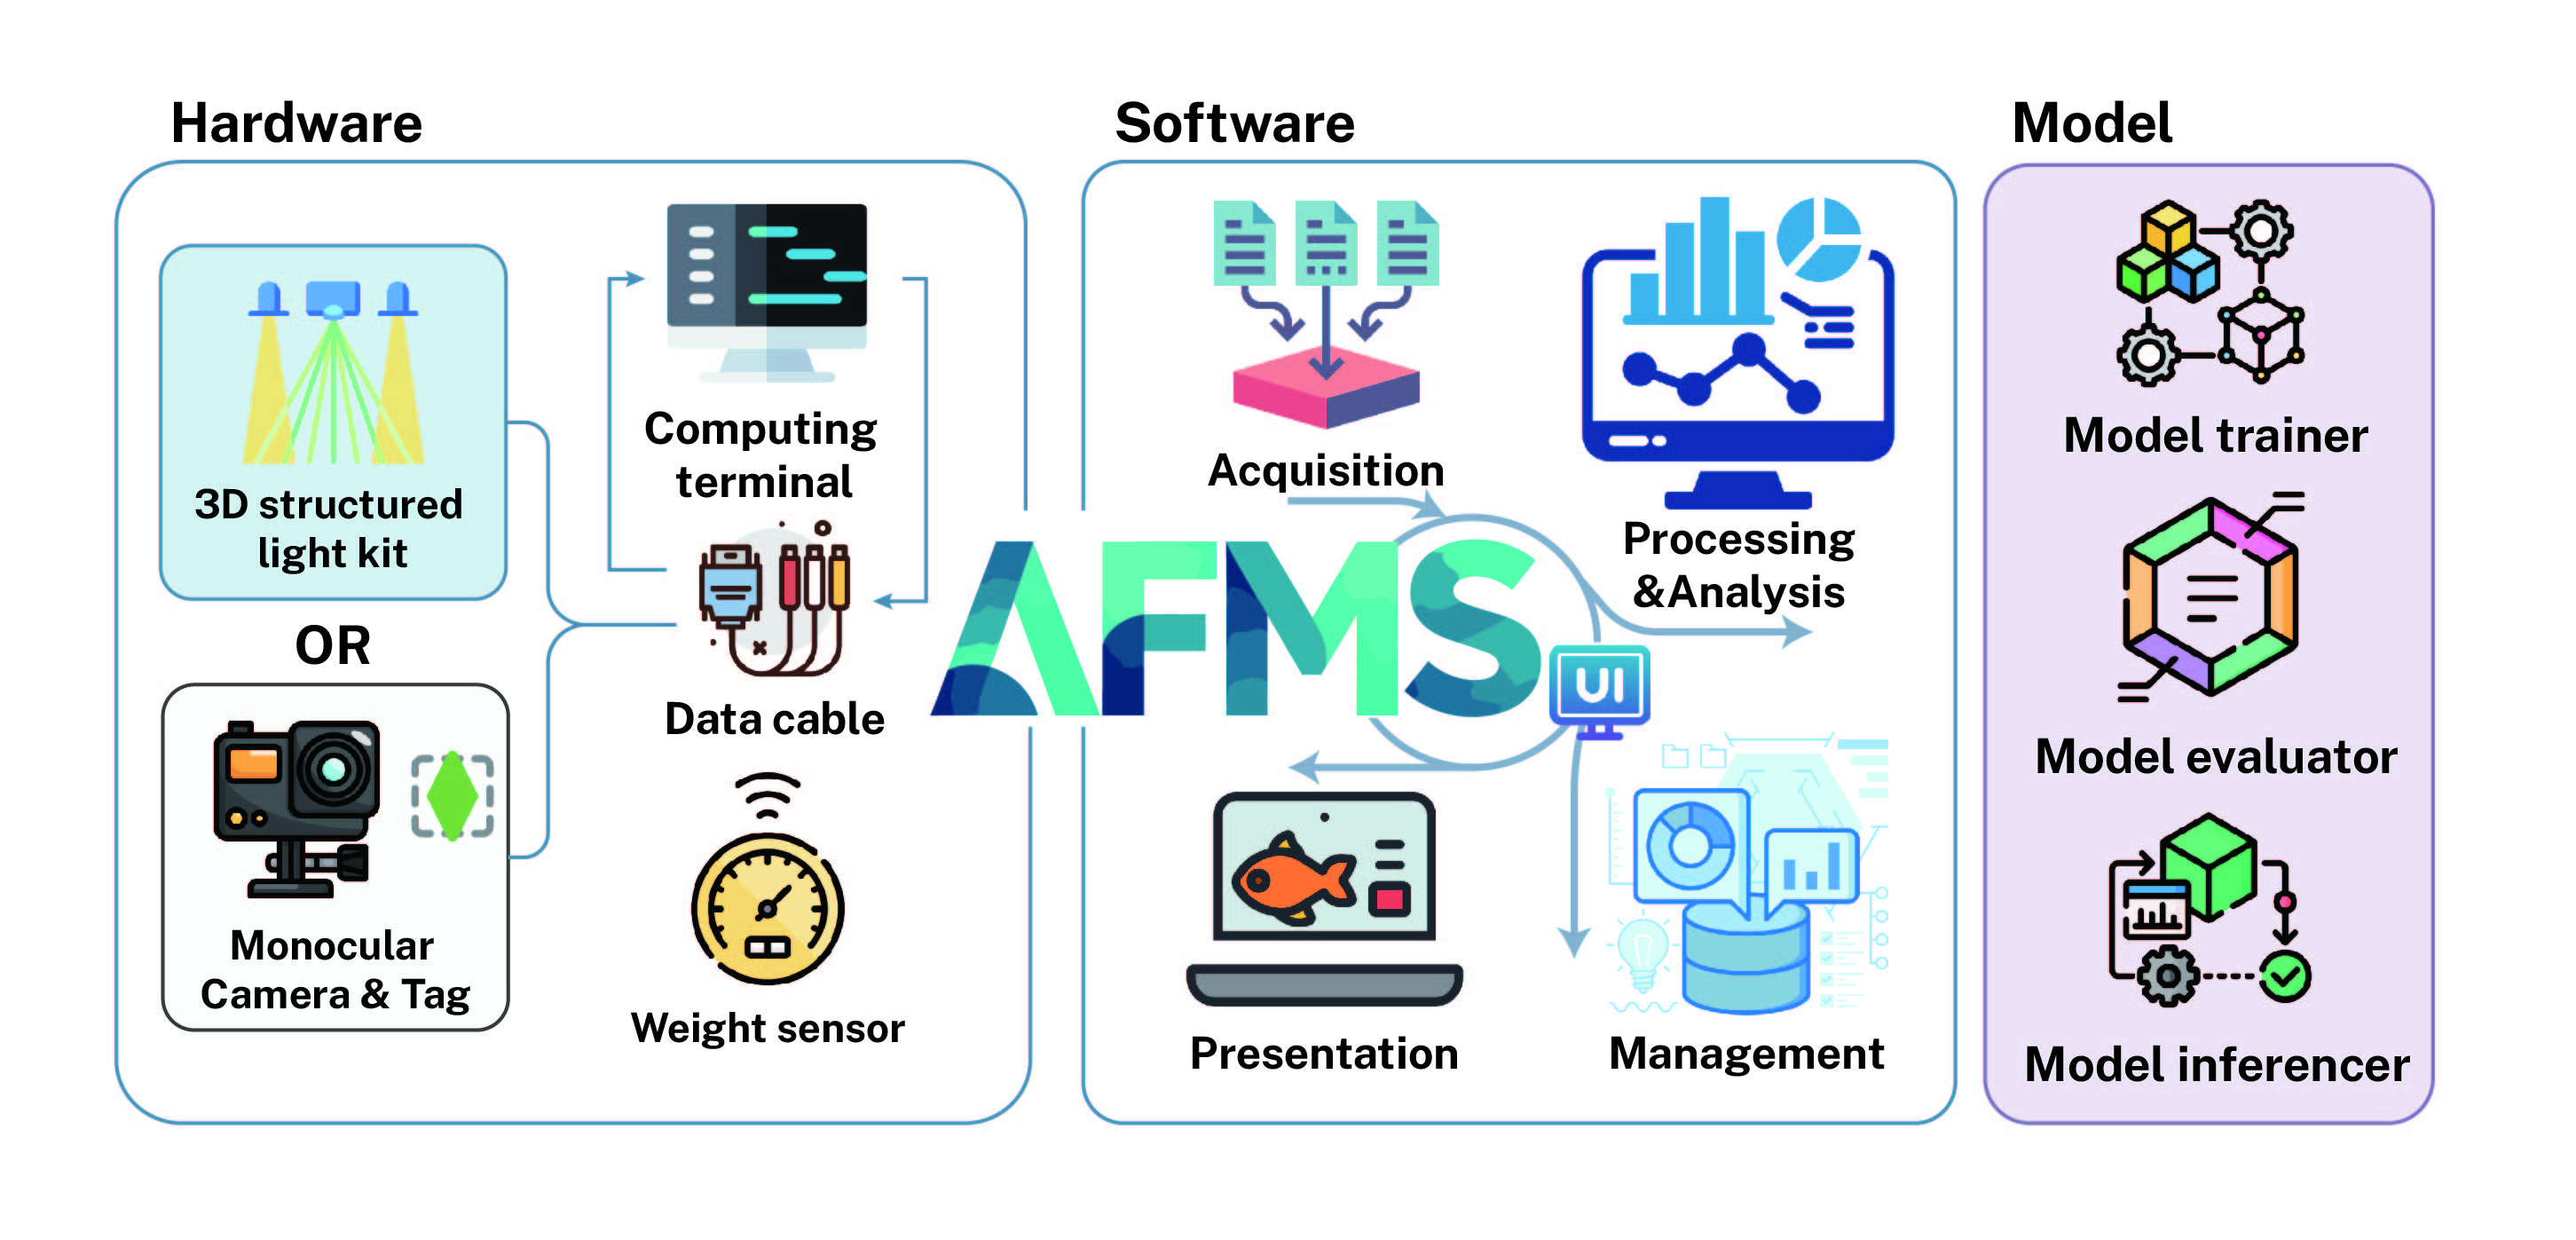
\includegraphics[width=\textwidth]{fig_system_architecture.jpg}
  \caption{AFMS system architecture. The framework separates acquisition hardware, measurement software, and model development. The species protocol at the center connects all layers, providing species-specific measurement definitions to every module.}
  \label{fig:system_architecture}
\end{figure}

The acquisition layer supports structured-light depth capture for real-space measurement \citep{veinidis2023reconstruction} and physical-tag-based calibration as a low-cost alternative. The software layer provides detection, landmark estimation, phenotype calculation, quality control, batch processing, and data export. The model layer is separated from the measurement software; it generates pre-trained model assets that can be imported into AFMS without changing the software architecture.

\subsection{Minimal species protocol}

The core innovation of AFMS is the minimal species protocol: a compact YAML record that defines what a species is and what to measure, without specifying how to detect or calculate. The protocol contains landmark definitions, landmark order, optional skeleton topology, measurement primitives (lines, angles, ratios), trait calculation rules, quality-control thresholds, and scoring rules (Table~\ref{tab:protocol_schema}). This declarative approach differs from traditional per-species coding patterns \citep{navarro2016imafish,he2024measurement} and aligns with configuration-driven designs in other biological imaging domains \citep{gonzalez2023phytooracle}.

\begin{table}[htbp]
  \centering
  \caption{Conceptual schema of a minimal species protocol. The protocol defines measurement semantics; the framework handles detection, calculation, and export.}
  \label{tab:protocol_schema}
  \small
  \begin{tabular}{p{0.28\textwidth}p{0.62\textwidth}}
    \toprule
    Protocol element & Role in AFMS \\
    \midrule
    Species metadata & Species identifier, display name, and target aquaculture animal type. \\
    Model assets & Pre-trained detector and landmark model paths. \\
    Landmark definitions & Species-specific anatomical landmarks with semantic names. \\
    Landmark order & Stable index order shared by annotation, training, inference, and measurement. \\
    Skeleton/topology & Optional landmark connections for visualization and consistency checking. \\
    Measurement primitives & Lines, angles, and ratios used to calculate phenotype traits. \\
    Scoring rules & Weighted quality scores for measurement traits using logistic functions. \\
    Quality-control thresholds & Minimum landmark confidence, missing-point tolerance, and validity checks. \\
    Display metadata & Names, labels, and display information for the user interface. \\
    \bottomrule
  \end{tabular}
\end{table}

Critically, the protocol is not a model configuration file. It does not specify backbone architectures, loss functions, or optimizer schedules. Instead, it defines measurement semantics: which landmarks to detect, which connections to draw, which lines and angles to calculate, and which quality rules to apply. The framework validates the protocol at load time through six semantic checks (verifying that every phenotype line references valid landmarks, every scoring rule references valid phenotype definitions, and every skeleton connection points to existing landmarks), ensuring that the protocol is self-consistent before any inference begins. Representative protocol examples are provided in Supplementary File S1.

The protocol simultaneously serves two roles. During model generation, a trainer reads the protocol and auto-generates species-specific detection and keypoint-estimation configurations by populating fixed architecture templates with protocol-defined landmark counts, skeleton structures, and dataset paths (Fig.~\ref{fig:model_workflow}). During runtime, the same protocol drives model loading, inference, landmark interpretation, phenotype calculation, quality control, scoring, and data export: all without species-specific conditional logic in the codebase.

\begin{figure}[htbp]
  \centering
  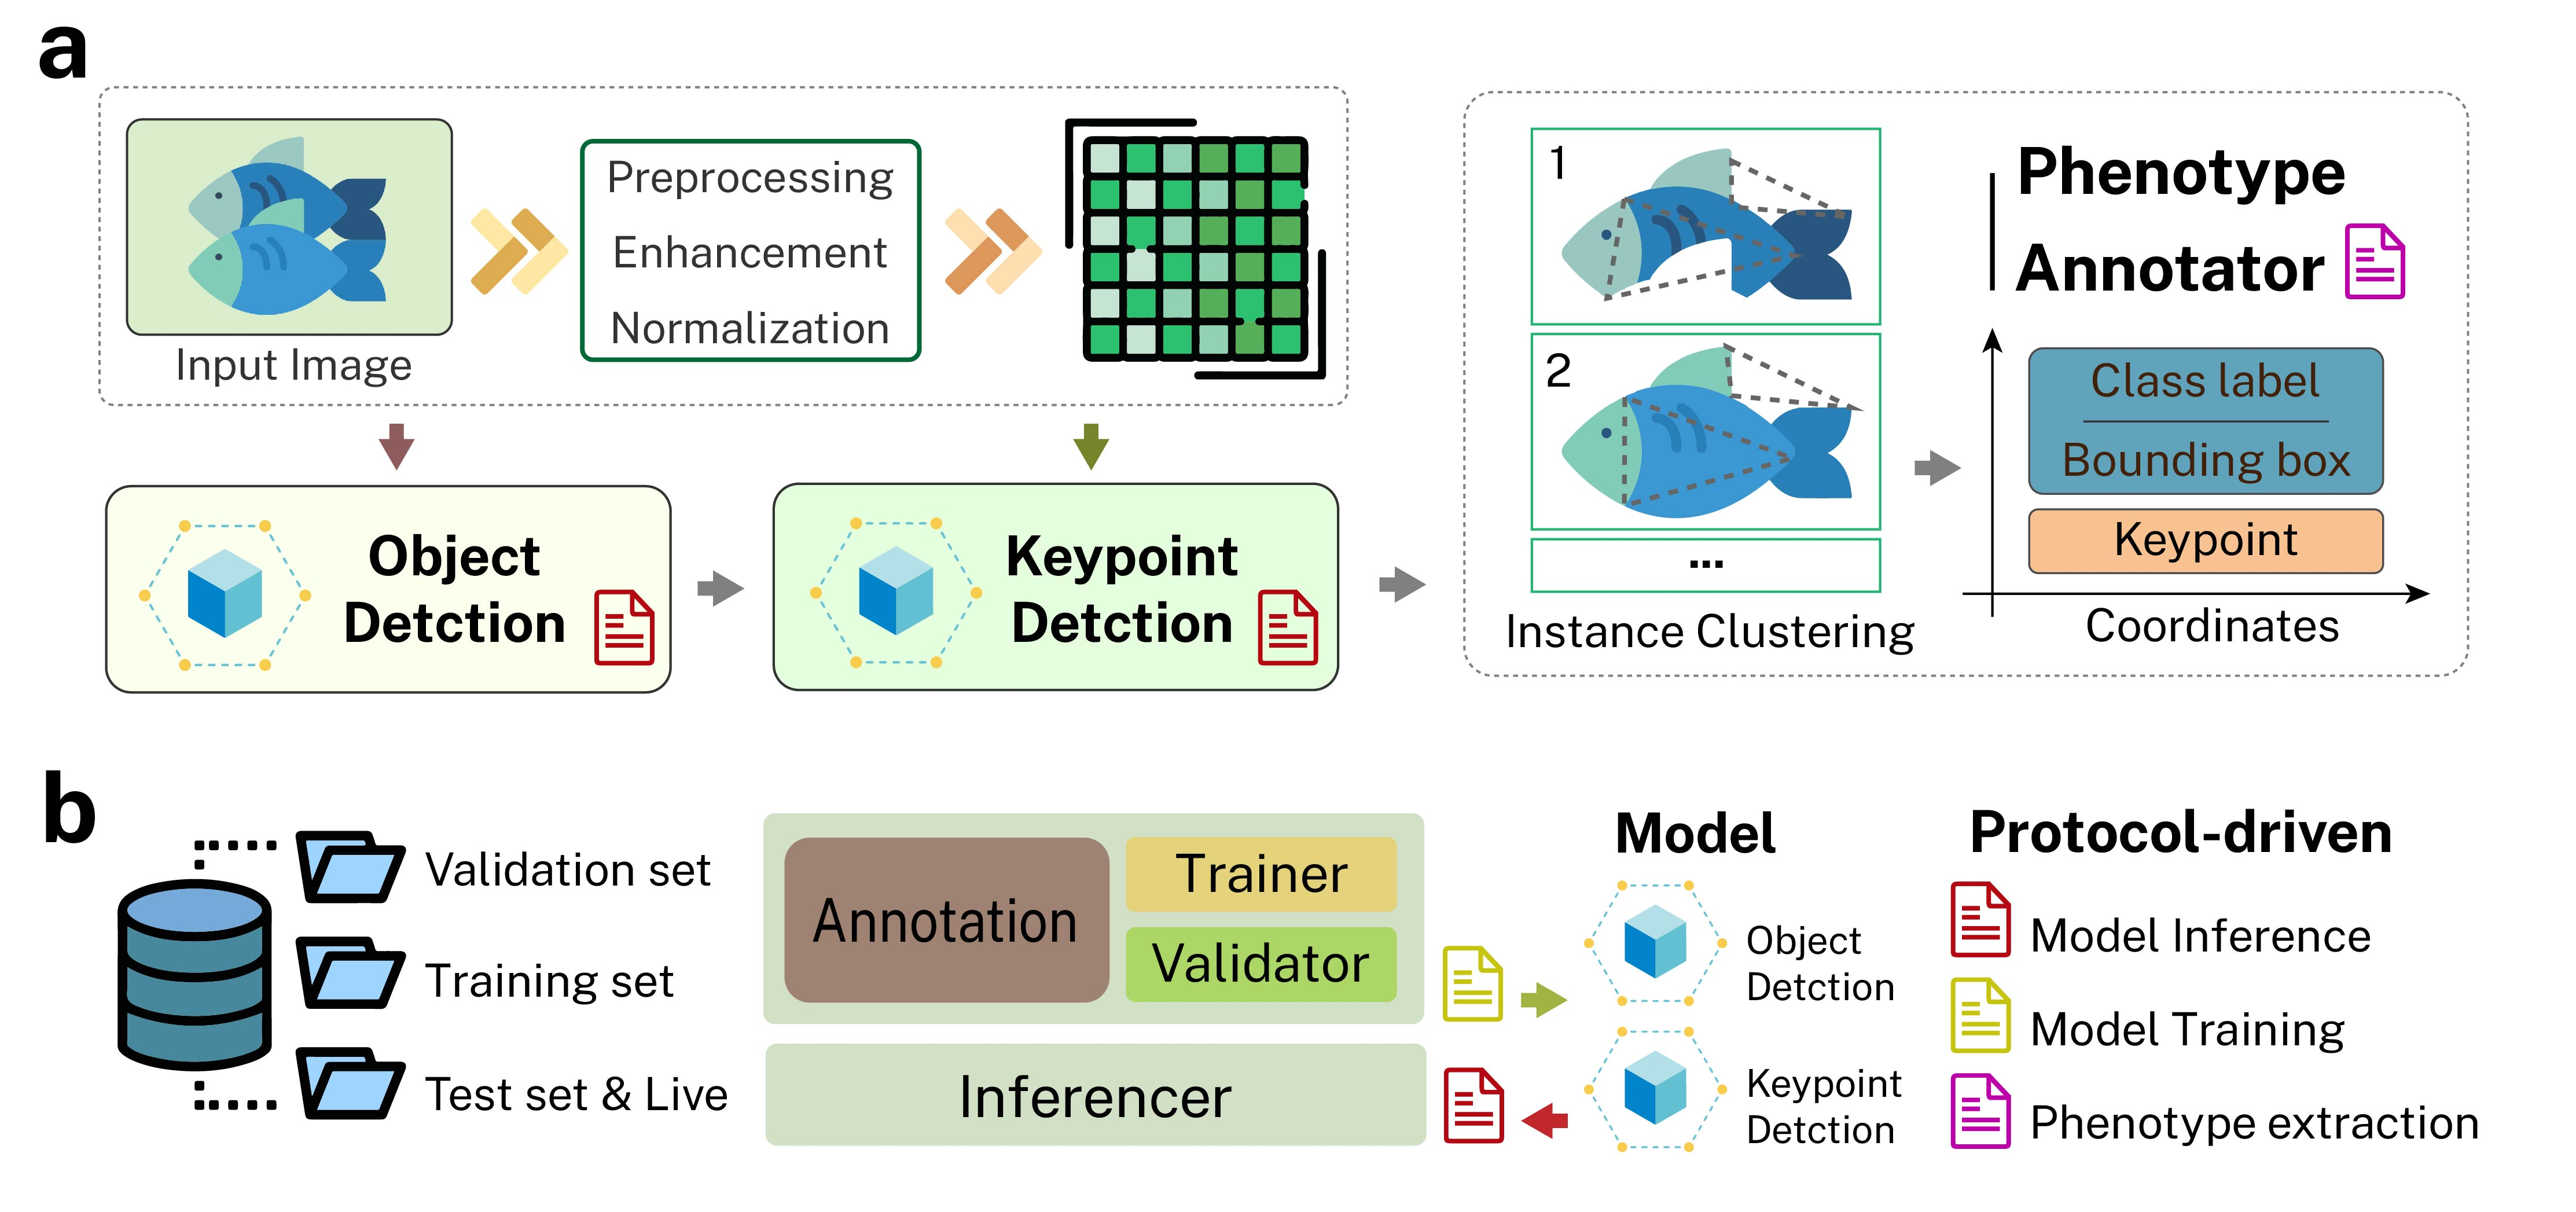
\includegraphics[width=\textwidth]{fig_model_trainer_workflow.jpg}
  \caption{Protocol-guided model generation and deployment workflow. The same YAML protocol guides training config generation on the left and runtime inference/measurement on the right.}
  \label{fig:model_workflow}
\end{figure}

Table~\ref{tab:workflow_comparison} compares the traditional development workflow with the AFMS protocol-driven workflow, illustrating the reduction in both code modification and required programming expertise.

\begin{table}[htbp]
  \centering
  \caption{Comparison of traditional and AFMS protocol-driven species adaptation workflows.}
  \label{tab:workflow_comparison}
  \small
  \begin{tabular}{p{0.30\textwidth}p{0.30\textwidth}p{0.30\textwidth}}
    \toprule
    Aspect & Traditional workflow & AFMS protocol workflow \\
    \midrule
    New species adaptation & Modify model configs, inference scripts, measurement functions, and export logic & Define one YAML protocol ($\sim$20 lines) \\
    Measurement rule change & Edit Python code & Edit YAML \texttt{phenotype} section \\
    Model upgrade (e.g.\ RTMPose-S to -L) & Change model config and inference code & Change ONNX path in protocol \\
    Scoring rule change & Edit scoring code & Edit YAML \texttt{scoring} section \\
    Programming required & Python & None (declarative YAML) \\
    \bottomrule
  \end{tabular}
\end{table}

\subsection{Species adaptation workflow}

For a new species, AFMS follows a protocol-first adaptation workflow:

\begin{enumerate}
  \item Define species metadata, landmark names, order, and optional topology in a protocol file.
  \item Annotate target images using the protocol-defined landmark semantics.
  \item Generate training configurations automatically from the protocol.
  \item Train species-specific detection and landmark models.
  \item Export model assets to ONNX.
  \item Import the protocol and ONNX assets into AFMS.
  \item Run inference, measurement, quality control, and phenotype export: all driven by the protocol.
\end{enumerate}

The purpose of this workflow is to avoid rewriting the core runtime for every species. Species adaptation is performed by updating the protocol and model assets, while the inference service, measurement engine, quality-control module, export module, and user interface remain shared. For all five tested species, no core runtime code modification was required. This contrasts with conventional approaches where each new species demands changes across the software stack \citep{liu2024fishphenokey,he2024measurement}.

\subsection{Multi-modal measurement}

AFMS supports three measurement modalities, all driven by the same protocol-defined measurement rules (Fig.~\ref{fig:depth_module}). In pixel-space mode, line distances and angles are calculated directly from image landmark coordinates. In physical-tag mode, rectangular reference tags in the scene provide scale calibration, converting pixel distances to physical units. In structured-light 3D mode, depth information from a multi-sensor module enables real-space geometric measurement \citep{veinidis2023reconstruction}.

\begin{figure}[htbp]
  \centering
  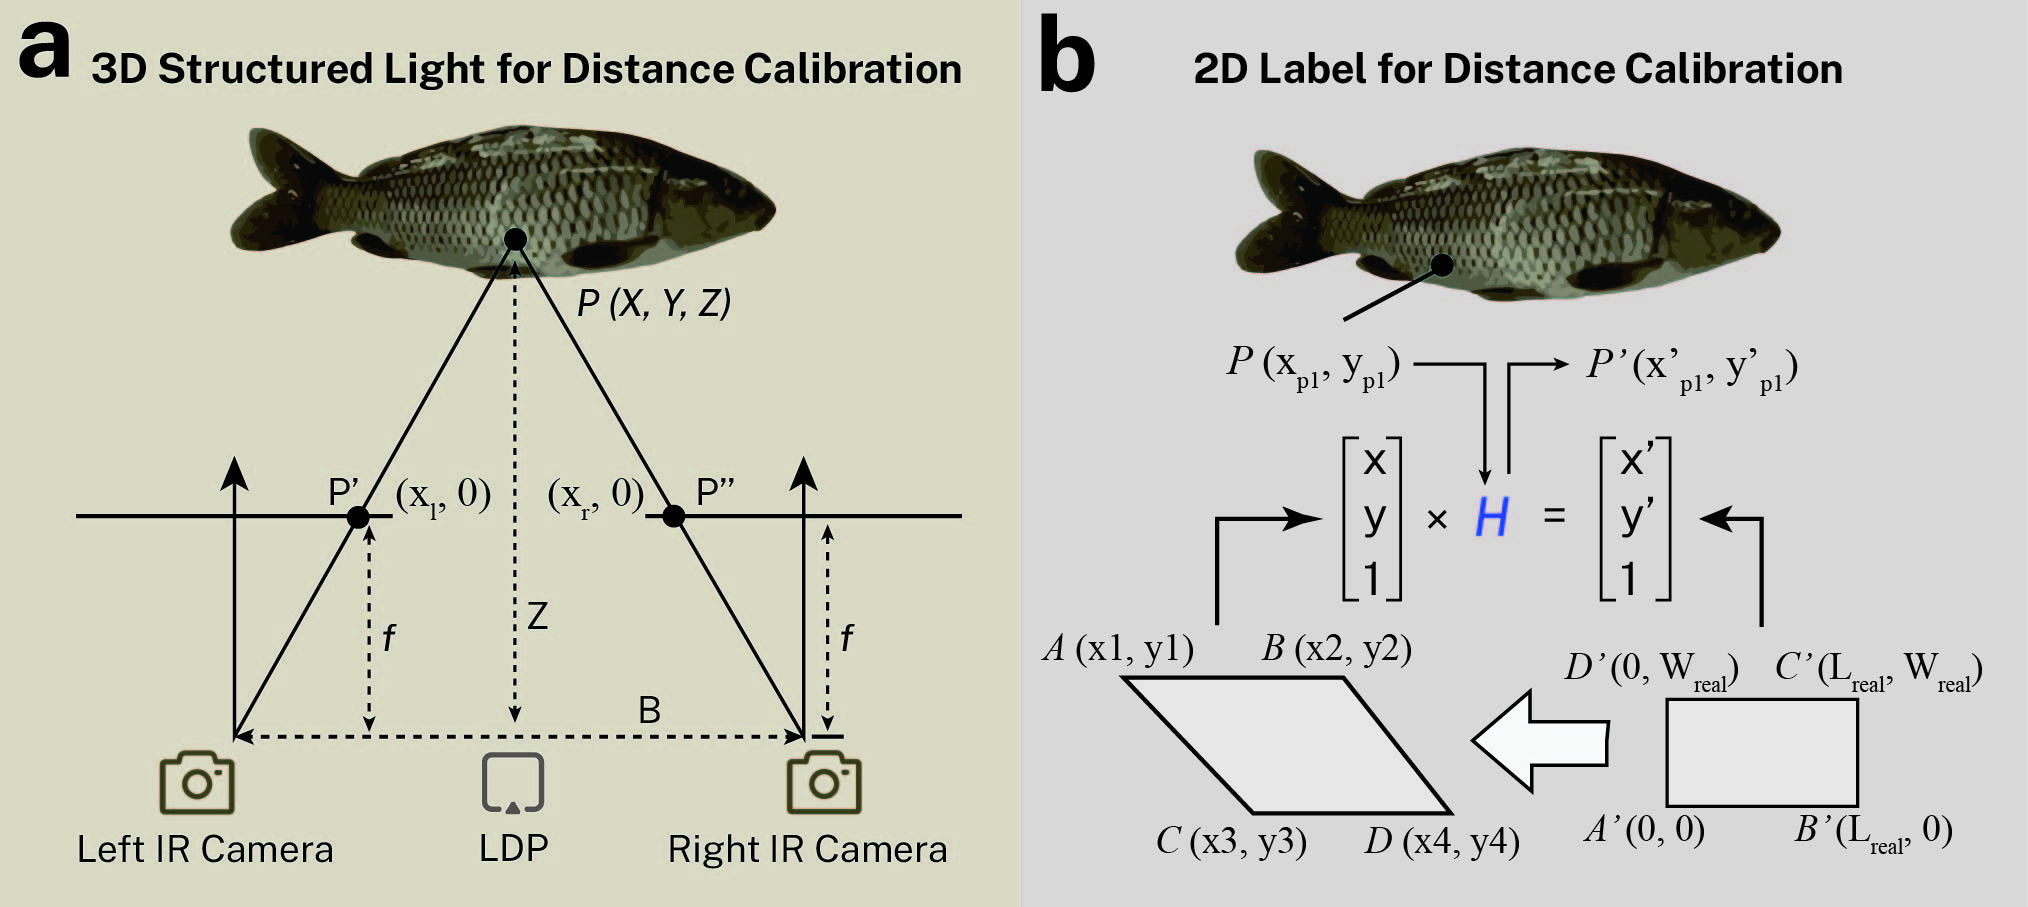
\includegraphics[width=0.80\textwidth]{fig_structured_light.jpg}
  \caption{Multi-modal measurement architecture. Protocol-defined measurement rules operate in three modes: pixel-space (2D), physical-tag-calibrated, and structured-light 3D. The depth module and tag module are interchangeable measurement backends driven by the same protocol.}
  \label{fig:depth_module}
\end{figure}

For structured-light measurement, a landmark pixel $p_i=(u_i,v_i)$ with depth $d_i$ is converted to camera-space coordinates:

\begin{equation}
  \mathbf{X}_i =
  \left(
  \frac{(u_i-c_x)d_i}{f_x},
  \frac{(v_i-c_y)d_i}{f_y},
  d_i
  \right),
\end{equation}

where $f_x$ and $f_y$ are focal lengths and $c_x$ and $c_y$ are principal point coordinates. Protocol-defined line and angle traits are then computed in 3D space:

\begin{equation}
  L_{ij}^{3D} = \lVert \mathbf{X}_i - \mathbf{X}_j \rVert_2,
  \qquad
  A_{ijk} =
  \cos^{-1}
  \left(
  \frac{(\mathbf{X}_i-\mathbf{X}_j)\cdot(\mathbf{X}_k-\mathbf{X}_j)}
  {\lVert \mathbf{X}_i-\mathbf{X}_j\rVert_2\lVert \mathbf{X}_k-\mathbf{X}_j\rVert_2}
  \right).
\end{equation}

The key architectural property is that the protocol defines measurement rules once, and the framework automatically adapts them to the available measurement backend. A breeder specifying ``measure the distance between landmarks P1 and P6'' does not need to know whether the calculation will be performed in pixels, tag-calibrated units, or 3D coordinates: the framework selects the appropriate backend based on the available sensor data. This separation of measurement intent from implementation is analogous to the abstraction layer design in modular phenotyping pipelines \citep{gonzalez2023phytooracle}.

\subsection{Model training and evaluation}

Detection models were implemented using RTMDet and keypoint models using RTMPose within the OpenMMLab ecosystem \citep{lyu2022rtmdet,jiang2023rtmpose,chen2019mmdetection,mmpose}. Datasets followed the COCO annotation format \citep{lin2014coco}. These models are replaceable perception components within AFMS rather than the main contribution; their role is to provide species-specific perception modules that can be exported to ONNX \citep{onnx} and deployed by the AFMS runtime.

The current implementation was evaluated on five taxa with distinct aquaculture body plans: common carp, Chinese mitten crab, red swamp crayfish, largemouth bass, and northern snakehead. The datasets contained 2697 images and 2907 annotated objects in total (Table~\ref{tab:datasets}). Detection was evaluated using COCO mAP and mAP@0.5. Keypoint estimation was evaluated using PCK, AUC, and NME. These metrics are reported as evidence that perception modules are adequate for downstream phenotyping, not as a claim that AFMS introduces a new detection or pose-estimation model. Multi-species keypoint benchmarks in aquaculture \citep{liu2024fishphenokey} and animal pose estimation surveys \citep{lin2025keypoint} provide broader context for these results.

\begin{table}[htbp]
  \centering
  \caption{Datasets used to demonstrate cross-species adaptation.}
  \label{tab:datasets}
  \small
  \resizebox{\textwidth}{!}{%
  \begin{tabular}{llrrrrr}
    \toprule
    Species & Scientific name & Landmarks & Train images & Val. images & Train objects & Val. objects \\
    \midrule
    Carp & \textit{Cyprinus carpio} & 13 & 868 & 217 & 1015 & 243 \\
    Chinese mitten crab & \textit{Eriocheir sinensis} & 12 & 348 & 90 & 350 & 90 \\
    Red swamp crayfish & \textit{Procambarus clarkii} & 3 & 140 & 35 & 158 & 39 \\
    Largemouth bass & \textit{Micropterus salmoides} & 12 & 266 & 67 & 279 & 68 \\
    Northern snakehead & \textit{Channa argus} & 7 & 532 & 134 & 531 & 134 \\
    \bottomrule
  \end{tabular}
  }
\end{table}

Batch-processing stability was evaluated on 1591 largemouth bass samples in an operational setting conducted by breeding practitioners. The benchmark recorded per-sample processing duration, success or failure status, and operator pause points. Failures were classified as detection failures (no target detected), keypoint estimation failures (landmark confidence below threshold), or acquisition failures (corrupted image data).

\section{Results}

\subsection{AFMS: a protocol-driven multi-species phenotyping platform}

AFMS is organized as a three-layer system with the protocol record at its center (Fig.~\ref{fig:system_architecture}). The acquisition layer provides structured-light depth capture and optional physical-tag calibration. The software layer contains 14 modules (inference, phenotype calculation, quality control, scoring, data export, and user interface), all of which read species-specific definitions from the protocol registry at runtime. The model layer generates ONNX assets that are loaded by the runtime through protocol-defined paths. Unlike earlier multi-species tools that embed species logic in code \citep{navarro2016imafish,he2024measurement}, AFMS resolves all species-specific behavior through a single registry.

The training-to-deployment pipeline (Fig.~\ref{fig:model_workflow}) shows how the same YAML protocol connects model generation and runtime measurement. On the training side, the protocol drives automatic generation of detection and keypoint-estimation configurations. On the runtime side, the same protocol drives model loading, landmark interpretation, phenotype calculation, scoring, and structured export. This unified pipeline reduces the engineering effort typically required to transition from model development to deployed phenotyping \citep{gonzalez2023phytooracle}.

\subsection{Multi-modal measurement driven by a single protocol}

AFMS supports three measurement modalities (pixel-space, physical-tag-calibrated, and structured-light 3D), all driven by the same protocol-defined measurement rules (Fig.~\ref{fig:depth_module}). Fig.~\ref{fig:depth_experiment} shows representative measurement outputs in both structured-light 3D mode and physical-tag mode. The structured-light capability builds on coded-light 3D reconstruction principles \citep{veinidis2023reconstruction} while integrating them within a unified protocol-driven framework.

\begin{figure}[htbp]
  \centering
  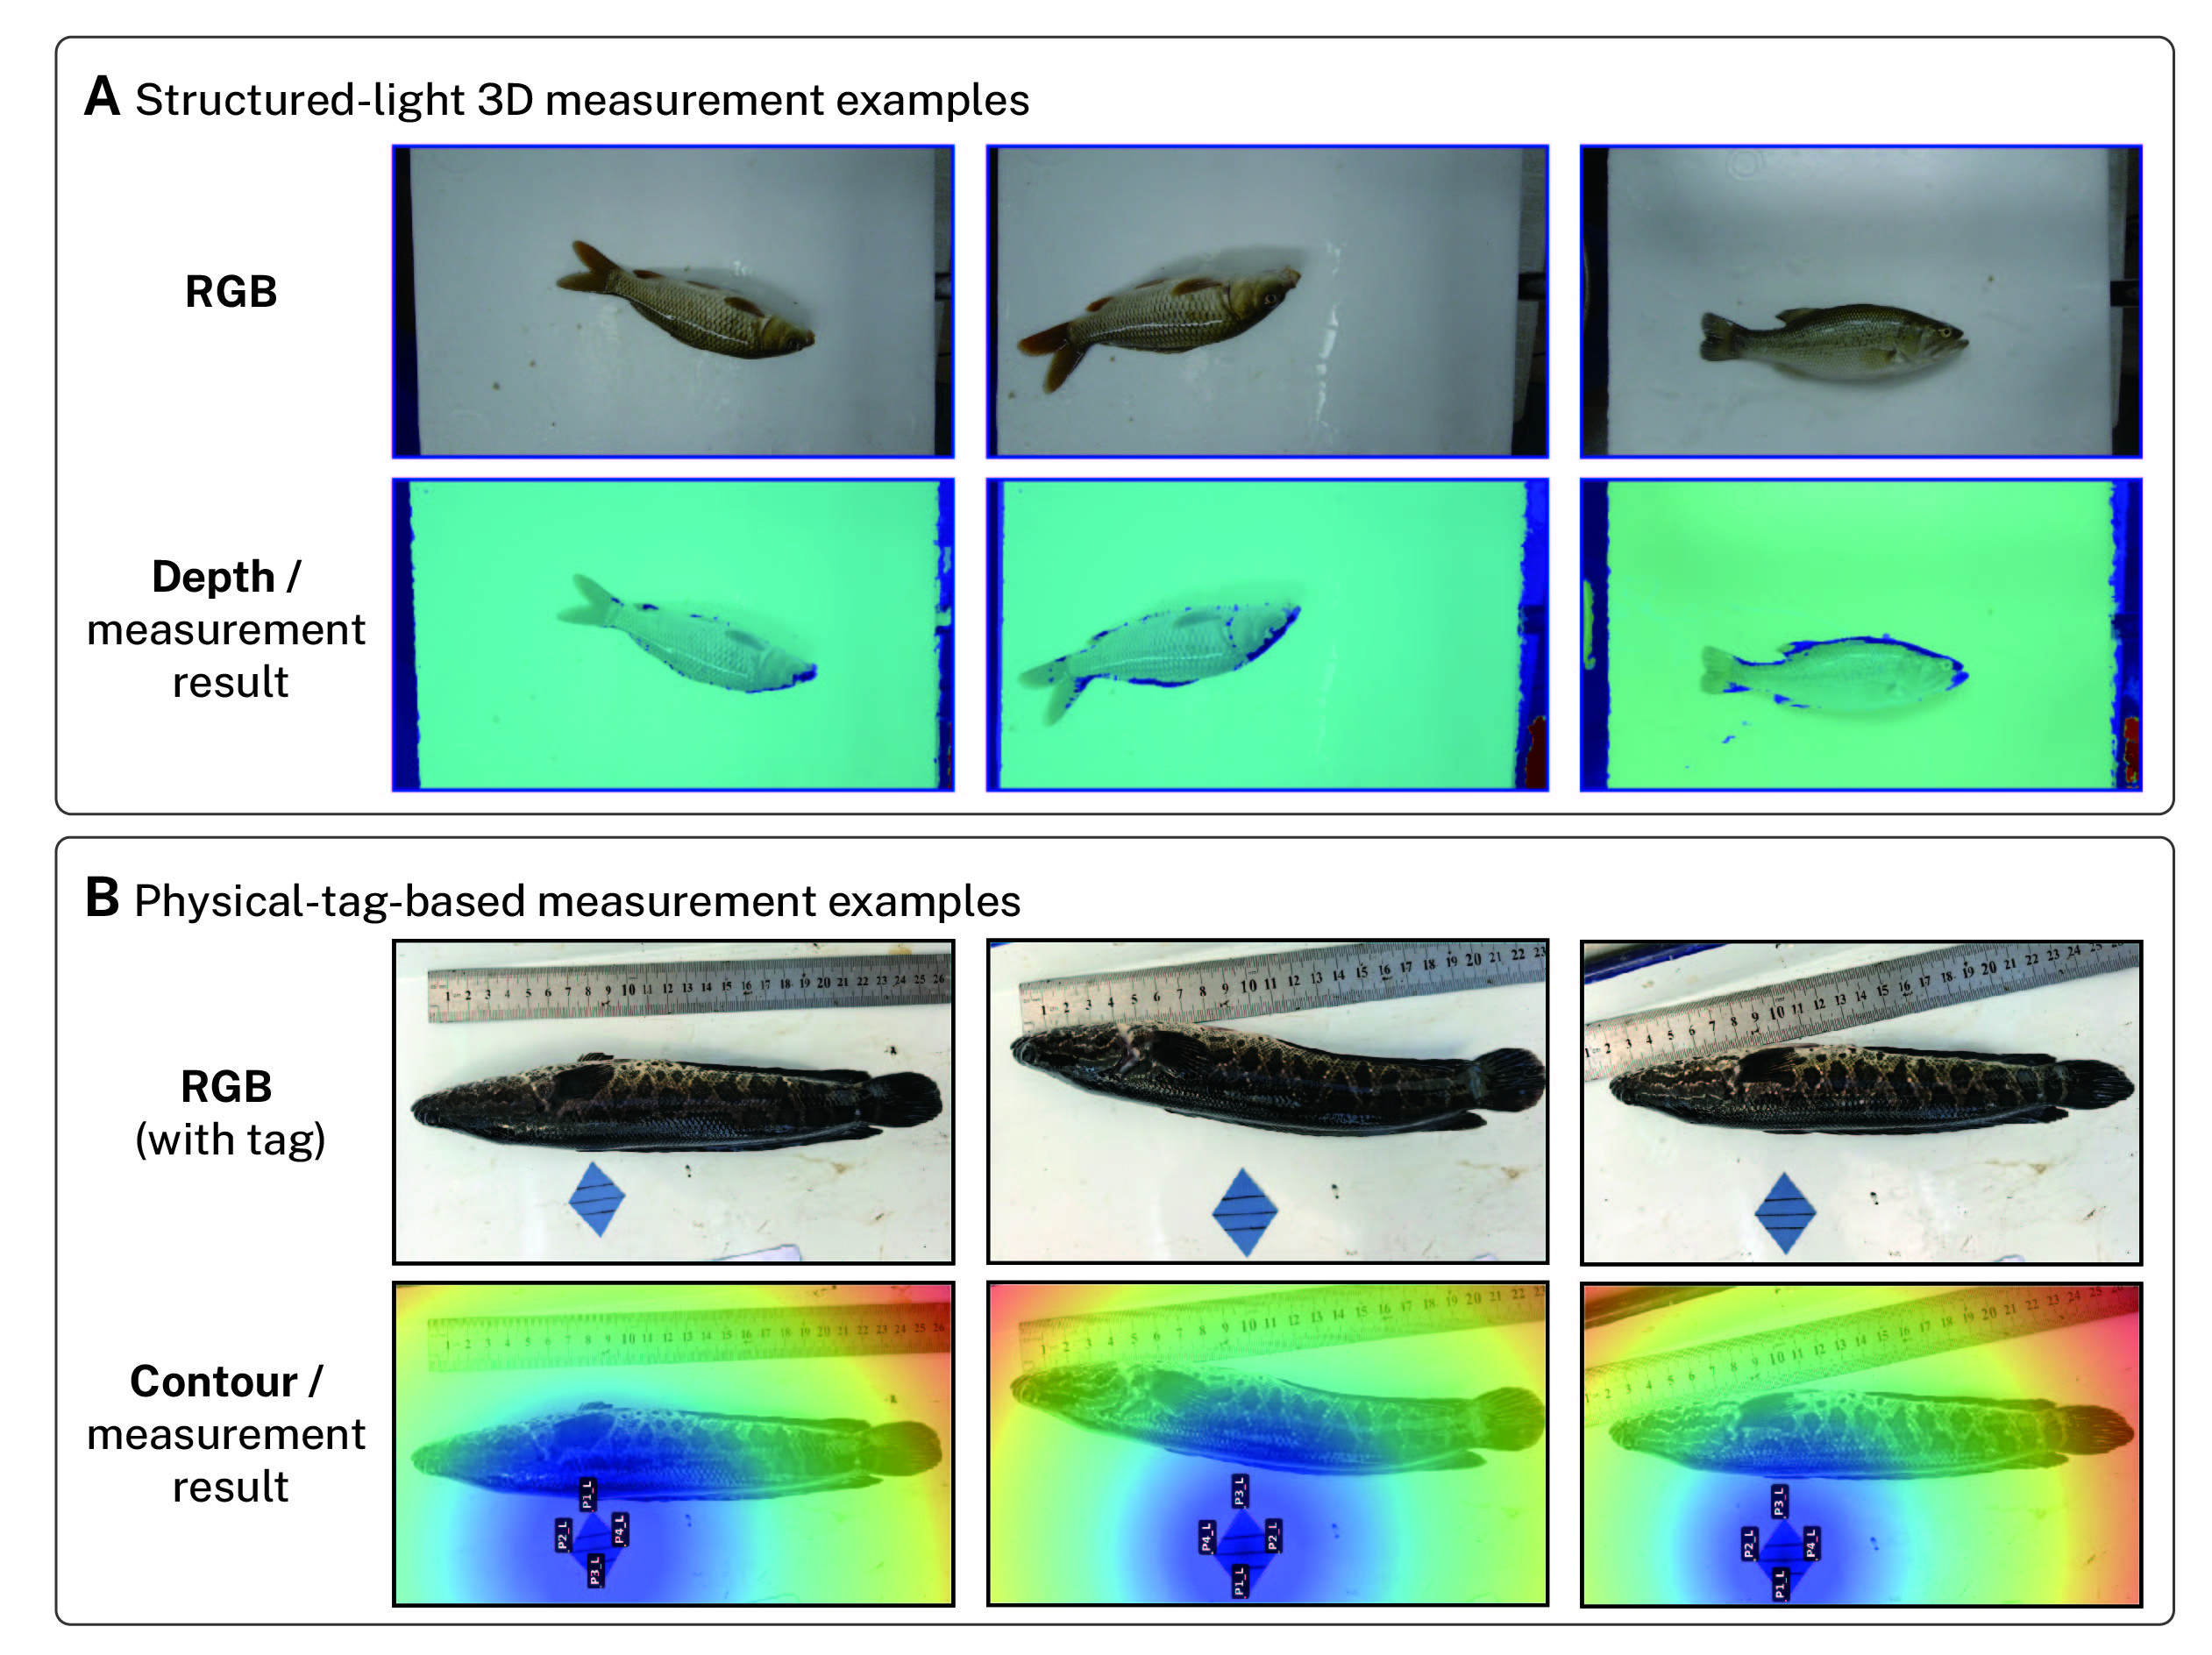
\includegraphics[width=\textwidth]{fig_structured_light_experiment.jpg}
  \caption{Representative measurement outputs in two modes. (A) Structured-light 3D measurement: RGB images (upper row) and depth-derived measurement results (lower row). (B) Physical-tag-based measurement: RGB images with reference tags (upper row) and contour-like measurement maps (lower row). Both modes are driven by the same protocol definition.}
  \label{fig:depth_experiment}
\end{figure}

The protocol-defined trait rules (line distances between landmarks, angles at landmark triples) operate identically across all three modes. Measurement intent is defined once in the protocol; the framework selects the appropriate coordinate system based on available sensor data. This multi-modal capability means the same protocol supports 3D measurement with structured-light hardware and field measurement with printed reference tags.

\subsection{Protocol-driven adaptation: five species, zero code modification}

The core evidence for protocol generality is that five morphologically diverse taxa share the same runtime codebase without core runtime code modification. Species differences were handled through protocol files and species-specific model assets. Table~\ref{tab:adaptation_loop} shows the adaptation status for all five species, confirming that protocol definition, model generation, ONNX deployment, and runtime loading are complete for each species, with no core runtime code modification required. Existing multi-species benchmarks \citep{liu2024fishphenokey} and generic measurement models \citep{he2024measurement} target multiple species but still require per-species model retraining or parameter adjustment; AFMS further reduces this overhead by unifying the measurement logic itself.

\begin{table}[htbp]
  \centering
  \caption{Protocol-driven species adaptation status. All five species share the same runtime without code modification.}
  \label{tab:adaptation_loop}
  \small
  \resizebox{\textwidth}{!}{%
  \begin{tabular}{lcccccc}
    \toprule
    Species & Protocol-defined landmarks & Model generated & ONNX deployment & Runtime loading & Traits measured & Core runtime code modification \\
    \midrule
    Carp & Yes & Yes & Yes & Yes & Protocol-defined & None \\
    Chinese mitten crab & Yes & Yes & Yes & Yes & Protocol-defined & None \\
    Red swamp crayfish & Yes & Yes & Yes & Yes & Protocol-defined & None \\
    Largemouth bass & Yes & Yes & Yes & Yes & Protocol-defined & None \\
    Northern snakehead & Yes & Yes & Yes & Yes & Protocol-defined & None \\
    \bottomrule
  \end{tabular}
  }
\end{table}

The protocol differences among species are substantial (Table~\ref{tab:protocol_comparison}), confirming that the framework handles genuinely diverse measurement definitions rather than minor parameter variations. Carp and crab share similar landmark counts (13 and 12, respectively) but define different trait lines and scoring rules. Crayfish uses only 3 landmarks with semantic names (\texttt{tou1}, \texttt{zhonbu}, \texttt{wei1}) rather than positional labels, demonstrating that the protocol operates at the semantic level rather than the parameter level. Snakehead defines 5 angle traits, while crab defines none.

\begin{table}[htbp]
  \centering
  \caption{Protocol comparison across five species. Substantial differences in landmark count, naming convention, and measurement rules confirm semantic-level protocol control.}
  \label{tab:protocol_comparison}
  \small
  \begin{tabular}{lcccccl}
    \toprule
    Species & Landmarks & Lines & Angles & Ratios & Skeleton & Naming convention \\
    \midrule
    Carp & 13 & 19 & 2 & 1 & 16 & Positional (P1--P12, PH) \\
    Crab & 12 & 17 & 0 & 1 & 16 & Positional (P1--P12) \\
    Crayfish & 3 & 2 & 1 & 1 & 2 & Semantic (\texttt{tou1}, \texttt{zhonbu}, \texttt{wei1}) \\
    Bass & 12 & 17 & 0 & 1 & 16 & Positional (P1--P12) \\
    Snakehead & 7 & 10 & 5 & 1 & 7 & Positional (P1--P7) \\
    \bottomrule
  \end{tabular}
\end{table}

In the runtime codebase, all species-specific behavior is resolved through the protocol registry. The inference engine loads models from protocol-defined paths, the phenotype calculator iterates over protocol-defined lines and angles, the scoring service applies protocol-defined weights, and the export module uses protocol-defined output fields. No species-specific conditional branches exist in any of these modules.

\subsection{Perception module validation}

The protocol-guided training workflow produced detection and keypoint-estimation modules for all five species (Table~\ref{tab:metrics}). Detection mAP@0.5 ranged from 0.955 to 1.000, and keypoint PCK ranged from 0.687 to 0.974. Four of five species achieved PCK above 0.927, comparable to fish keypoint benchmarks in the literature \citep{liu2024fishphenokey,ge2024cefish}, indicating that the perception modules are adequate for downstream phenotyping. The crayfish results (PCK 0.687) reflect the challenges of sparse 3-landmark topology on a small dataset (140 training images), rather than a limitation of the protocol architecture. Similar data-scarcity challenges have been noted in animal pose estimation surveys \citep{lin2025keypoint}.

\begin{table}[htbp]
  \centering
  \caption{Validation metrics for protocol-generated perception modules. These values confirm that modules are adequate for downstream phenotyping; they are not presented as cross-species model rankings.}
  \label{tab:metrics}
  \small
  \resizebox{\textwidth}{!}{%
  \begin{tabular}{lrrrrrrrr}
    \toprule
    Species & Val. images & Val. objects & Protocol landmarks & Protocol traits & mAP & mAP@0.5 & PCK & NME \\
    \midrule
    Carp & 217 & 243 & 13 & 22 & 0.871 & 0.988 & 0.928 & 0.134 \\
    Chinese mitten crab & 90 & 90 & 12 & 18 & 0.762 & 0.981 & 0.974 & 0.097 \\
    Red swamp crayfish & 35 & 39 & 3 & 4 & 0.682 & 0.955 & 0.687 & 0.095 \\
    Largemouth bass & 67 & 68 & 12 & 17 & 0.687 & 0.970 & 0.932 & 0.106 \\
    Northern snakehead & 134 & 134 & 7 & 16 & 0.787 & 1.000 & 0.967 & 0.028 \\
    \bottomrule
  \end{tabular}
  }
\end{table}

\subsection{Operational batch-processing validation}

In an operational test conducted by breeding practitioners, AFMS processed 1591 largemouth bass samples over 118 minutes of continuous operation (Fig.~\ref{fig:stress_batch}). Of these, 1572 completed successfully and 19 failed, corresponding to a 98.8\% success rate. The average processing duration was 4.45\,s per sample. Sixteen operator pause periods were recorded during the run, reflecting real-world usage conditions rather than a simulated benchmark.

\begin{figure}[htbp]
  \centering
  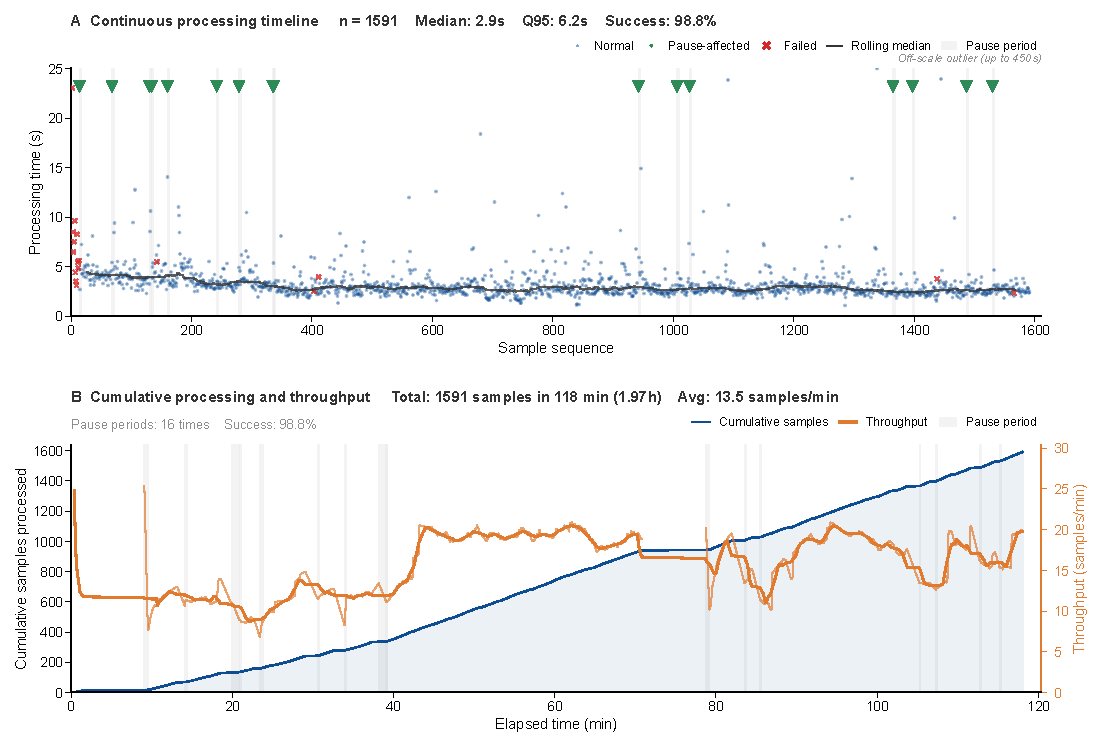
\includegraphics[width=\textwidth]{fig_stress_batch_combined.pdf}
  \caption{Operational batch-processing test. (A) Continuous processing timeline during the 1591-sample run. Points show per-sample processing time, failed samples, and operator pause events. Of the 19 failures, 6 occurred within $\pm$5 samples of pause events, suggesting that post-pause recovery periods carry a slightly elevated failure risk. (B) Cumulative processing and rolling throughput during the same batch test. Operator pause periods create plateaus in cumulative throughput; processing resumes after intervention.}
  \label{fig:stress_batch}
\end{figure}

This test validates that the protocol-driven architecture supports sustained batch phenotyping under real-world operating conditions. The protocol registry loads species definitions, the inference engine processes samples through protocol-defined models, the phenotype calculator applies protocol-defined measurement rules, and the export module writes structured records: all without manual intervention between samples. To our knowledge, this is among the first reports of operational batch-processing throughput and success rate for a multi-species phenotyping system in aquaculture, as most prior studies report model accuracy rather than end-to-end pipeline reliability \citep{navarro2016imafish,he2024measurement,tonachella2022fishial}.

\section{Discussion}

\subsection{Protocol-driven architecture as a reusable phenotyping interface}

The Results demonstrate that a minimal species protocol can serve as the single interface for multi-species phenotyping, enabling five morphologically diverse taxa to share a single runtime without code modification. This section discusses what this result means for aquaculture phenotyping and for the broader computer-vision community.

The protocol-driven architecture represents a shift from model-centric thinking to infrastructure-centric thinking. The computer-vision community typically evaluates contributions by model accuracy: a new backbone, a new loss function, a new attention mechanism. AFMS does not claim to introduce a better model. Its RTMDet and RTMPose components are established architectures \citep{lyu2022rtmdet,jiang2023rtmpose}. The contribution is the architecture that connects these models to phenotyping workflows through a protocol-defined semantic layer. In long-term breeding and production contexts, models will be upgraded and replaced over time; what must remain stable is the interface between measurement intent and model implementation. This perspective aligns with trends in other biological phenotyping domains, where modular, configurable pipelines are increasingly adopted over monolithic per-species solutions \citep{gonzalez2023phytooracle}.

\subsection{Why extensibility matters in aquaculture}

Aquaculture animals are morphologically diverse. A body-axis measurement tool designed for one fish cannot directly represent the carapace and appendage structure of crabs, and a sparse crayfish landmark set cannot be treated as a simple variant of a 12-landmark fish topology. The protocol comparison in Table~\ref{tab:protocol_comparison} quantifies this diversity: landmark counts range from 3 to 13, trait definitions range from 4 to 22, and naming conventions span positional labels and semantic names.

AFMS addresses this diversity by allowing each species to define its own landmark semantics and measurement rules while sharing the same runtime architecture. Measurement intent is defined in the protocol; the framework handles detection and calculation. This separation allows anatomical measurement intent to be represented independently from inference and measurement implementation. Recent multi-species fish keypoint benchmarks \citep{liu2024fishphenokey} and generic measurement models \citep{he2024measurement} have begun addressing cross-species generalization at the model level, but AFMS tackles the same challenge at the architecture level by decoupling measurement logic from implementation.

\subsection{Multi-modal measurement for diverse production conditions}

The three measurement modalities (pixel-space, tag-calibrated, and structured-light 3D) address different production conditions. Pixel-space measurement provides rapid relative comparisons when absolute physical units are not required. Physical-tag calibration offers low-cost physical-unit measurement using only a camera and printed reference tags, suitable for field conditions where structured-light hardware is unavailable. Structured-light 3D measurement provides a real-space measurement backend for controlled acquisition settings.

All three modes are driven by the same protocol definition. This means a breeding program can start with low-cost tag-based measurement and upgrade to structured-light 3D without redefining measurement rules or modifying application code. Structured-light techniques have demonstrated high accuracy for fish 3D reconstruction \citep{veinidis2023reconstruction}, and their integration within a protocol-driven framework makes them accessible to breeding programs without specialized computer vision expertise.

\subsection{Limitations and future work}

Several limitations should be acknowledged. First, the current validation covers five species across three taxonomic orders, but more extreme body plans (such as bivalves, jellyfish, or sessile organisms) have not been tested. The protocol design supports arbitrary landmark counts and semantic naming, but empirical validation on additional taxa is needed. Second, training still requires COCO-format annotation, which may require annotation tools or assistance for users unfamiliar with the format. Third, the current protocol supports lines, angles, and ratios as measurement primitives; extending to new primitives such as area or curvature requires one-time framework-level additions rather than per-species changes, but this extension has not yet been implemented. Fourth, the structured-light measurement module has been integrated but not independently validated for sensor accuracy against ground-truth physical measurements.

Future work will focus on expanding the protocol library to additional aquaculture taxa, integrating individual identification \citep{zhang2026fishfaceid} and breeding-database linkage for longitudinal phenotype tracking, developing more user-friendly protocol-authoring interfaces and deployment documentation, and evaluating farm-scale deployment under diverse production conditions \citep{tonachella2022fishial}.

\section{Conclusions}

This work demonstrates that a minimal species protocol can serve as the single interface for multi-species aquaculture phenotyping. New species are added by defining measurement intent (landmarks, trait connections, quality rules), while the same runtime handles inference, phenotype calculation, quality control, and structured export without core runtime code modification. Across five morphologically diverse aquaculture taxa spanning three taxonomic orders, the same runtime processed all species with no core runtime code modification, achieving detection mAP@0.5 from 0.955 to 1.000 and an operational batch-processing success rate of 98.8\% over 1591 samples.

AFMS reduces species adaptation from repeated software redevelopment toward protocol-level definition. The bottleneck in scaling aquaculture phenotyping is not model accuracy but the coupling between measurement intent and software implementation \citep{gonzalez2023phytooracle}. By externalizing this coupling into declarative protocol records, AFMS provides a reusable infrastructure for adapting computer-vision-based phenotyping across species \citep{liu2024fishphenokey}. Future work will expand the protocol library, integrate individual identification \citep{zhang2026fishfaceid} and breeding-database linkage, and evaluate farm-scale deployment to bridge the gap between laboratory phenotyping and production-scale aquaculture management.

\section*{Declaration of competing interest}

The authors declare that they have no known competing financial interests or personal relationships that could have appeared to influence the work reported in this paper.

\section*{Data and code availability}

The AFMS source code, protocol files for all five species, and trained model assets are available from the corresponding authors upon reasonable request. The datasets used in this study contain images of breeding populations with ongoing commercial and research value; they are not publicly released at this time but may be made available on a collaborative basis. Final figure assets and supporting data are maintained in the project repository.

\section*{Acknowledgements}

Acknowledgement text to be completed by the authors before submission.

\bibliographystyle{elsarticle-num}
\bibliography{references}

\end{document}
